\chapter{System Evaluation}\label{chap:eval}
One of the aims stated for this study as listed in the Chapter~\ref{sec:Introduction} was to write a Python application with scalability in mind. Therefore this chapter is devoted to present a 1000 feet view of the application so that the implementation described in prior chapters could be taken as only one of possibilities to realise the intended system characteristics and functionality.  The second section presents a discussion of SmartNotes application metrics taken using such a benchmarking tools like \texttt{autobench} or \texttt{siege} and statistics from the Google App Engine dasboard. This chapter together with Chaper~\ref{cha:conclusions} summarises the results for the subject of this study. 

\section{Final result presentation}\label{sec:result}
Created application has a client-server architecture which segments were presented in Figure~\ref{fig:smartnotes_components} and has the features of flexibility, scalability and security what was described in Section~\ref{sec:gae} subsections. The web interface of SmartNotes is a simple internationalized application that provides general informations about the project and lets the iterated users access its functionality. Currently that includes only creating a SmatNotes account by using the Google Account as described in Section~\ref{subsec:ismartnotes_activation} and receiving an activation key. That process is straight forward and it is presented in Figure~\ref{fig:sn_web_interface}. Finally the users can pass the activation code to  the iSmartNotes application to take the advantage of synchronisation feature. It allows the users as described in Section~\ref{sec:functionality_descr} to work on their notes and perform a synchronisation whenever they want to. The main iSmartNotes window is presented in Figure~\ref{fig:ismartnotes_window}. It has a simple text area where the notes can be edited and a \texttt{Sync} button that dependently on the network connectivity will perform synchronisation on local machine or additionally using the SmartNotes network infrastructure. This basic attempt realises the functionality  excluding sharing and grouping notes which are extensions to the present functionality and will be added to the SmartNotes application beyond the focus and implementation completed in this study. It can be clearly noted that it cant compete with such a applications like this described in Section~\ref{sec:popular_apps} which was presenting and comparing popular notes taking applications. On the other hand that related work was used as a inspiration for  creating a scalable fundament that could be later become more complex by adding additional functionality. That way the gathered experience can become further expanded and make the SmartNotes more attractive to the users. The created blog, feedback form and hosing the source code on well known Open source service does not only point to gather users attention but also to find developers who like the idea behind it and collaborate on it. 

Chosen technologies provide a well documented and truly active environment with the relatively low access barrier allowing to get involved in a short time. Some of chosen solutions like Django or Mercurial could become substituted with their equivalents among different language environments or using the Java language as a universal binding for those tools\footnote{Java programming language is wide know for its dynamic curve of development and great thread management. This features ore few on the list motivating the existence of such a projects as JRuby, Jython or Quercus which are the Java implementations of respectively  Ruby, Python and PHP languages. That way different runtimes can be used on one common environment taking advantage from all of Java features.}.       
\begin{figure}[ht]
  \begin{center}
    \subfigure[\textbf{SmartNotes homepage with basic informations and authentication}.]{\label{fig:sm_main}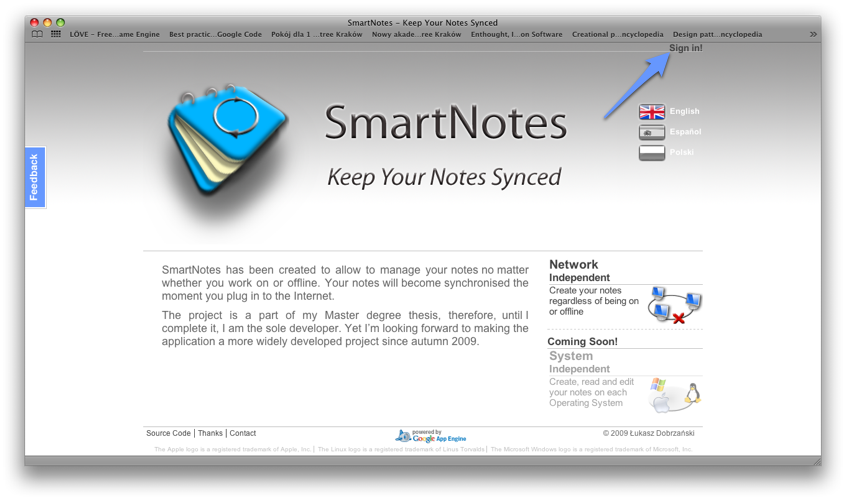
\includegraphics[scale=0.5]{img/SNmain_page.png}}
    \subfigure[\textbf{Authentication using the Google account}.]{\label{fig:sm_signin}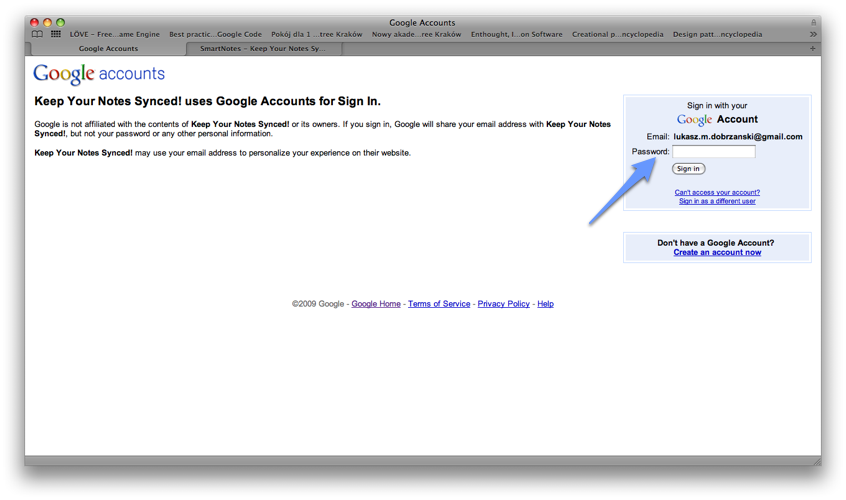
\includegraphics[scale=0.24]{img/SN_signin.png}}
    \subfigure[\textbf{Obtaining the SmartNotes activation key}.]{\label{fig:sm_getSNkey}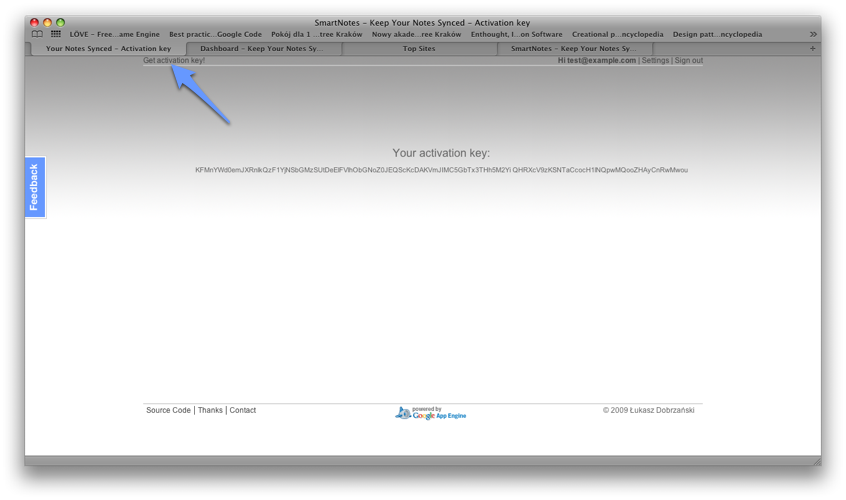
\includegraphics[scale=0.24]{img/SNget_activation_key.png}}
  \end{center}
  \caption{The view on the public web-based SmartNotes interface with basic informations regarding the project and authentication.}
  \label{fig:sn_web_interface}
\end{figure}
That direction of development seams to become recently popular and is worth of attention. However the chosen set of components including:
 \begin{itemize}
 	\item{Google App Engine -- as a platform providing scalable infrastructure and few additional useful API's for mailing, imaging or remote task queues.}
	\item{Django famework -- one of Python web frameworks which attracts more and more developers trough its clean architecture, usability available out of the box and strong community.}
	\item{Mercurial -- pure Python version control system with well designed support for HTTP protocol and zero cost of administration.}
 \end{itemize} 
 is one of is very powerful allowing to carry out the desired functionality with easiness for further development. That aspect should be always remembered during any design process and when choosing between concurrent solutions. That combined with system streamlining  for concrete use cases  determines why entire system concept is highly desirable when building scalable systems.
        
\begin{figure}[ht]
\begin{center}
\includegraphics[scale=0.5]{img/SN_ismartnotes_window.pdf}
\caption{The view on the iSmartNotes application window.}
\label{fig:ismartnotes_window}
\end{center}
\end{figure}

\section{Performance tests}\label{sec:performance} 